\usepackage{graphicx} % Required for inserting images
\usepackage{xcolor}
\usepackage{enumitem}
\usepackage{amsmath}
\usepackage{tikz}
\usepackage{fullpage}
\usepackage{mathtools}

\usetikzlibrary{arrows,shadows,positioning}
\usepackage{pgf-umlsd}

\newcounter{diagram}
\newcounter{step}
\counterwithin*{step}{diagram}
\newcommand\nextstep{\refstepcounter{step}\thestep: }
\newcommand\resetstep{\refstepcounter{diagram}}

\newcommand{\ramc}[1]{\textcolor{cyan}{#1}}
\newcommand{\eepromc}[1]{\textcolor{red}{#1}}
\newcommand{\ramt}[1]{#1}
\newcommand{\eepromt}[1]{#1}

% \bibliographystyle{plain}
% \usepackage[style=numeric,backend=biber,sorting=none]{biblatex}
% \addbibresource{refs.bib}

\usepackage[breaklinks,hyperindex,colorlinks,anchorcolor=black,citecolor=black,filecolor=black,linkcolor=black,menucolor=black,urlcolor=black,pdftex]{hyperref}


\definecolor{midblue}{rgb}{0,0,.7}
\hypersetup{
  colorlinks=true,
  linkcolor=midblue,
  citecolor=midblue,
  urlcolor=midblue
}

\title{Security Protocol Project \\ \Large{Design Proposal}}
\author{Felix M\"older \\ s1022118
\and Maximilian Pohl \\ s1103073
\and Bart Veldman \\ s1017975}
\date{\today}

\begin{document}

\maketitle

% Project Information sheet:
% http://www.cs.ru.nl/~erikpoll/spp/javacard_project.pdf


\section{Use Cases}
Our group decided to design, develop and implement the E-Purse system.
This system consists of the following components:
\begin{itemize}
    \item Smart cards
    \item Reload terminals
    \item POS (point-of-sale) terminals
    \item Initialization terminals
    \item A back-end
\end{itemize}
The issuer of the cards uses the initialization terminal to initialize a new card and deliver the initialized card to the end-user.
At every reload terminal, the user can load money on their smart card and can pay for goods and services at every POS terminal that are supplied by salesmen.
An example application for this system is a university canteen.
Students can load money on their student card at reload terminals.
Later, they can pay for lunch and food at the POS terminals in the university canteen.
We will define the following use cases:
\begin{enumerate}[label={UC\arabic*:}, ref={UC\arabic*}, leftmargin=3\parindent]
    \item \label{uc:person} The card is initialized at an initialization terminal once before provided to the end-user.
    
    \item \label{uc:reload} At a reload terminal, the end-user can increase the balance of the smart card by paying with cash or with a bank card.
    
    \item \label{uc:payment} At the POS-terminal, the end-user can pay for goods and services with the smart card.
    A user can use a POS terminal, even if the terminal is not connected to the back-end (offline).

    \item A POS or reload terminal can be deactivated remotely with some delay (e.g., one week).
    
    \item The end-user can declare the card as lost or stolen, which results in the card being blocked.
    For the sake of simplicity of the protocol, we do not allow the unblocking of a blocked card.
    
\end{enumerate}
\subsection{Lifecycle}
The lifecycle of the smart-cards is depicted in Figure~\ref{fig:lifecycle}.
%In the \emph{Initial} state, the smart card consists only the raw program and no user data is loaded on the card yet.
In the \emph{Initial} state, the program is already loaded on the card, but no data exist yet.
In an actual application, the possibility to upload other applets or to remove existing once would already be disabled at this stage.

By uploading the required data onto the card, the card will move to the state \emph{Personalized}.
This is done with the initialization terminal and the initialization protocol as described in Section~\ref{sec:perProtocol}.
At this stage, the card is still in the possession of the card issuer.

By handing the card over to the end-user, the card transits to the \emph{Issued} state.
Internally to the card, this does not make a difference to the previous state.

We decide between two end states.
Either a card gets \emph{Blocked} because it was lost or stolen, or it moves to the \emph{End-of-Live} state, because it reached its expiration date or the transaction counter, which is explained later, overflows.
The two end states do not make a difference internally to the card, but the card can not be used anymore.

\begin{figure}
    \centering
    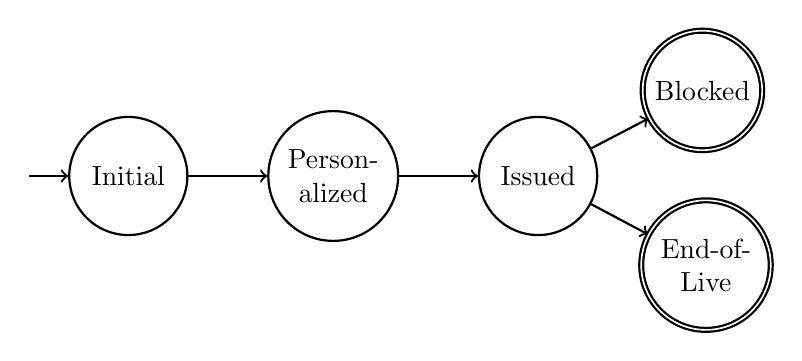
\begin{tikzpicture}[node distance=0mm and 1cm, thick, end/.style = {main, double}, main/.style = {draw, circle, align=center, minimum size=1.5cm}] 
\coordinate (start);
\node[main] (init) [right=0.5cm of start]{Initial}; 
\node[main] (person) [right=of init]{Person-\\alized}; 
\node[main] (issued) [right=of person] {Issued}; 
\node[end] (blocked) [above right=of issued] {Blocked}; 
\node[end] (eol) [below right=of issued] {End-of-\\Live};
\draw[->] (start) -- (init);
\draw[->] (init) -- (person); 
\draw[->] (person) -- (issued);
\draw[->] (issued) -- (blocked);
\draw[->] (issued) -- (eol);
\end{tikzpicture} 
    \caption{Lifecycle of the smart-card}
    \label{fig:lifecycle}
\end{figure}


\section{Attacker Model}\label{attackerModel}
To understand possible attack scenarios, we first have to list what a potential attack would like to achieve.
The goals of an attacker, i.e., the threats considered in our protocol, are:
\begin{enumerate}[label={T\arabic*:}, leftmargin=2\parindent, ref={T\arabic*}]
    \item \label{threat:increaseWithoutPaying}
    The end-user is interested in increasing its balance (which is stored on the card) without actually paying for it.
    
    \item \label{threat:payWithoutDecrease}
    The end-user is interested in forging a payment such that the POS terminal shows a succeeded transaction without the balance of the card actually decreased.
    
    \item \label{threat:denyPayment}
    The end-user is interested in denying having done a payment that actually happened, in order to get the money back.
    
    \item \label{threat:forgingPayments} The salesman is interested in forging payments by either 
    \begin{enumerate}[ref={\theenumi~\alph*}]
        \item \label{threat:inventNewPayments}
        inventing payments that never happened or
        \item \label{threat:alterPaymentDetails}
        by altering the details of payments that happened, such as the money-source and destination or the amount transferred.
    \end{enumerate}
        
    \item \label{threat:chargeMoreThanDisplayed}
    The salesman is interested in charging more money than shown on the terminal display (if there is any).

    \item \label{threat:invaldTermial} A third person is interested in operating unauthorized POS terminals to collect payment proofs and get the money from the institution operating the system, e.g., by inserting the collected payment proofs into the log of a valid terminal.

    \item \label{threat:stolenCard} A third person is interested in using a stolen or lost card to pay with it at POS terminals.
\end{enumerate}

% Power:
%   Active MITM
%   card tear (pulling it out of the terminal while operating)
We assume an attacker that is able to shut down the card and the terminal at any (precise) point in time, e.g., by tearing the card out of the terminal or by removing the power supply of the terminal, respectively.
Additionally, an attacker is capable of performing an active man-in-the-middle attack.
This means, it can read and alter any communication between the smart card and the terminal.

% TCB
%   Assume tamper-resistance
%   which persons do we have to trust?
On the other hand, we assume the smart cards and terminals to be tamper resistant.
This means, it is not possible for an attacker to extract key material from the card or terminal and that the software and data stored are integer and cannot be changed.
Still, we do not want the security of the whole system to be compromised in case of a single failure in this assumption.

Furthermore, we have to trust on the correctness of data fed to the terminals, e.g., the reload terminal being able to correctly count the cash inserted and that nobody tampers with the connection between the money counting machine and the terminal.
Likewise, we have to trust the clock signal the terminal provides to the card, as the card cannot keep track of time itself.
Moreover, we assume that communication between the back-end and the terminals is secure.

We also do not specifically secure the initialization step.
Securing the initialization is not needed, as this functionality is already disabled when the card is given to the end-user.
It is also impossible to create a valid card in case someone gets their hands on some uninitialized card, as this would require the knowledge of private secrets only known by the back-end.
We do not even have to trust the person initializing the cards too much, as the private key of the card is generated within the card and, given that the software was not tapered with, cannot be exported.
The person thus could create a lot of cards with no money on them, which is not too interesting as a business model.


\section{Security Requirements}
Our system will adhere to the following security requirements (SR's). After each SR we indicate which threat from Section~\ref{attackerModel} it aims to prevent.
\begin{enumerate}[label={SR\arabic*:}, leftmargin=3\parindent]

    % RELOAD TERMINAL
    \item \label{sr:cardAuthReload}
    The card authenticates the reload terminal. (\ref{threat:increaseWithoutPaying})
    \item \label{sr:reloadCardMessageAuth}
    A reload terminal message to a card is authenticated. (\ref{threat:increaseWithoutPaying})
    \item \label{sr:noReplayLoadingCard}
    A reload terminal's message increasing a card's balance is usable only once. (\ref{threat:increaseWithoutPaying})
    \item \label{sr:cardReloadMessageIntegrity}
    A breach of integrity in the communication between a card and a reload terminal is noticed. (\ref{threat:increaseWithoutPaying})
    \item \label{sr:cardReloadtransterAtomic}
    Money transfer between a card and reload terminal must behave atomic. (\ref{threat:increaseWithoutPaying})
    \item \label{sr:disableReload}
    A reload terminal can be deactivated remotely by trustful parties. (\ref{threat:increaseWithoutPaying})

    % POS TERMINAL
    \item \label{sr:POSAuthCard}
    A POS terminal authenticates the card. (\ref{threat:payWithoutDecrease})
    \item \label{sr:cardAuthPOS}
    The card authenticates the POS terminal. (\ref{threat:invaldTermial})
    \item \label{sr:POScardMessageAuth}
    A card's message to a POS terminal is authenticated. (\ref{threat:payWithoutDecrease})
    \item \label{sr:cardPOSMessageAuth}
    A POS terminal's message to a card is authenticated. (\ref{threat:chargeMoreThanDisplayed})
    \item \label{sr:noReplayDecreasingCard}
    A POS terminal's message decreasing a card's balance is usable only once. (\ref{threat:inventNewPayments})
    \item \label{sr:cardPOSMessageIntegrity}
    A breach of integrity in the communication between a card and a POS terminal is noticed. (\ref{threat:payWithoutDecrease}, \ref{threat:alterPaymentDetails})
    \item \label{sr:cardNonRepudiation}
    The owner of a card cannot deny a payment being made to a POS terminal. (\ref{threat:denyPayment})
    \item \label{sr:proofTransaction}
    A POS terminal collects proof of transactions. (\ref{threat:denyPayment})
    \item \label{sr:cardPOStransterAtomic}
    Money transfer between a card and POS terminal must behave atomic. (\ref{threat:payWithoutDecrease})
    \item \label{sr:disablePOS}
    A POS terminal can be deactivated remotely by trustful parties. (\ref{threat:invaldTermial})

    % CARD
    \item \label{sr:keyLeakage}
    When a key leaks, only that card should be affected, not other cards. (\ref{threat:increaseWithoutPaying}--\ref{threat:forgingPayments})
    \item \label{sr:disableCard}
    A card can be deactivated remotely by trustful parties. (\ref{threat:stolenCard})
\end{enumerate}

We decided against the following security requirements:
\begin{itemize}
    \item We do not encrypt the traffic between the card and the various terminals.
    The reason being that we do not see any relevant threat that would get mitigated by that and would therefore only complicate the protocol without a real improvement.
    We are unsure if there is any legal requirement to encrypt the traffic, e.g., for privacy reasons.
    If so, the protocol needs to be modified accordingly.
    
    \item We decided against the authentication of the cardholder (e.g., by PIN protection), as we took systems like the Dutch \emph{Chipknip} or the usage of the student identity card for paying in the university canteen in Germany as a model.

    \item We do not authenticate the card to the reload terminal, as we did not figure out any threat that could be mitigated by that.
    If someone loads money on a faked, expired, or otherwise invalid card, the money would be lost, as the card cannot be used at any POS terminal.
\end{itemize}


\section{Key Distribution and Protocols}
\subsection{Notation}
The following notation will be used throughout the section:
\begin{itemize}
    \item Private keys are lower case
    
    \item Public keys are capitalized
    
    \item The subscript indicates the owner (c: Card, p: POS, r: Reload, b: Back-end)
    
    \item Encryption will be notated as: $\textrm{Enc}_{\textrm{Key}}(\textrm{Message})$

    \item Decryption will be notated as: $\textrm{Dec}_{\textrm{Key}}(\textrm{Ciphertext})$
    
    \item Computation of a hash will be notated as: $\textrm{H}(\textrm{Message})$
    
    \item Certificates will be written as: $\textrm{Cert}_\textrm{owner}^\textrm{issuer}(\textrm{attributes})$
\end{itemize}


\subsection{Key and Certificate Distribution}

An overview of the keys used in the protocol can be found in Table~\ref{tab:keys}.
\begin{table}[h]
    \centering
    \begin{tabular}{|l|p{2cm}|p{1.5cm}|p{4.7cm}|p{2.7cm}|}
\hline
    Symbol & Name & Owner & Purpose & Origin \\
\hline
    $k_c$ & Private key of the card & Card & Authenticate at terminals and setup shared secret with them & Generated in the card \\
\hline
    $K_c$ & Public key of the card & Card & Authenticate at terminals and setup shared secret with them & Generated in the card \\
\hline
    $k_p$ & Private key of the POS terminal & POS & Authenticate at cards and setup shared secret with them & Generated in the terminal \\
\hline
    $K_p$ & Public key of the POS terminal & POS & Authenticate at cards and setup shared secret with them & Generated in the terminal \\
\hline  
    $k_r$ & Private key of the reload terminal & Reload terminal & Authenticate at cards and setup shared secret with them & Generated in the terminal \\
\hline
    $K_r$ & Public key of the reload terminal & Reload terminal & Authenticate at cards and setup shared secret with them & Generated in the terminal \\
\hline
    $k_b$ & Private key of the back-end, also called master key & back-end & Used to sign certificates of the cards, POS, and reload terminals & Generated in the back-end \\
\hline
    $K_b$ & Public key of the back-end & back-end & Stored on every smart card, POS, reload terminal to verify certificates & Generated in the back-end \\
\hline
\end{tabular}
    \caption{Keys used in the protocol}
    \label{tab:keys}
\end{table}

Table~\ref{tab:certs} gives an overview over all certificates used.
In order to synchronize all transactions with the back-end, the reload and POS terminals are required to connect to the back-end periodically.
We assume this period to be one week.
To enforce this, the certificates to authenticate the POS and reload terminals are valid for one week at most.
This makes it possible to deactivate any fraudulent terminal within one week at most, by not issuing any new certificate to it.
This assumes that the clock provided by the terminal is genuine.
If it is not, a terminal can use an old certificate and just provide some clock signal that is within the validity range of this old certificate.

Additionally, it enables blocking cards by distributing a certificate revocation list (CRL) to the POS terminals periodically (e.g., once a week).
As shown in Step~\ref{seq:payPOScheckCardCert} in the payment protocol, the POS checks if the certificate of the card is revoked by the most recent CRL\@.

\begin{table}[h!]
    \centering
    \begin{tabular}{|l|p{1.7cm}|p{1.5cm}|p{1.5cm}|p{4cm}|p{3cm}|}
\hline
    Symbol & Name & Owner & Issuer & Purpose & Content \\
\hline
    $\textrm{Cert}_c^b$ & Card \mbox{certificate} & card & Back end & Authenticate the card at POS terminals & Card ID, expiration date, \texttt{0x01}, signature \\
\hline
    $\textrm{Cert}_p^b$ & POS \mbox{certificate} & POS & Back end & Authenticate the POS to the card & POS ID, expiration date, \texttt{0x02}, signature \\
\hline
    $\textrm{Cert}_r^b$ & Reload \mbox{certificate} & reload terminal & Back end & Authenticate the reload terminal to the card & Reload ID, expiration date, \texttt{0x03}, signature \\
\hline
\end{tabular}
    \caption{Certificates used in the protocol}
    \label{tab:certs}
\end{table}

Certificates will have the structure as defined in Table~\ref{tab:certStructure}.
\begin{table}[h!]
    \centering
    \begin{tabular}{|p{8cm}|}
    \hline
        ID (card or terminal ID) \\
    \hline
        Expiration date \\
    \hline
        Public key of the certificate owner \\
    \hline
        One byte indicating the intended usage: \texttt{0x01}: card, \texttt{0x02}: POS terminal, \texttt{0x03}: reload terminal \\
    \hline
        $S = \textrm{Enc}_{k_b}$(H(all of the above)) \\
    \hline
    \end{tabular}
    \caption{General structure of the certificates used}
    \label{tab:certStructure}
\end{table}

To verify a certificate, the following steps will be taken:
\begin{itemize}
    \item Check the expiration date
    \item Check whether H(cert content) $\stackrel{?}{=} \textrm{Dec}_{K_b}$(signature $S$)
    \item Check if the usage byte (see Table~\ref{tab:certStructure}) matches
    \item The POS terminal additionally checks if the card ID is part of the most recent CRL\@.
\end{itemize}


\subsection{Security Protocols}
% TODO
% Skip agreeing on which programs to use.
% Verifying certificate: what does it mean?

\subsubsection{Personalization Protocol} \label{sec:perProtocol}
The Personalization Protocol depicted in Figure~\ref{fig:PersonProtocol} describes the steps taken for use case~\ref{uc:person}.
The Initialization Terminal functions as a channel for the back-end. 
The smart-card is given its ID and expiration date and generates its own public-private key-pair in steps~\ref{seq:InitDetailsToCard}--\ref{seq:InitGenKey}.
This ensures that only the card knows its private key. 
Additionally, the smart card receives the signature of its certificate from the back-end in steps~\ref{seq:InitSignBackEnd} and~\ref{seq:InitSignatureToCard}.
The protocol finishes with the smart card blocking its initialization functionality and sending a success message to the initialization terminal. 
After the initialization process, every smart card contains the following information:
\begin{itemize}
    \item The private key $k_c$ of the card
    \item The public key $K_c$ of the card
    \item The public key $K_b$ of the back-end
    \item The identification number of the card
    \item The expiration date on which the card expires
    \item A boolean specifying whether the card is blocked or not
    \item A boolean specifying that the card is initialized and can therefore not be initialized again
\end{itemize}

 \begin{figure}[h!]
     \centering
     \resetstep
\begin{sequencediagram}
    \newthread[white]{i}{i:Initialization Terminal}
    \newinst[3]{c}{c:Smart Card}
    \newinst[-14]{b}{b:Back end}

    \begin{call}
        {i}{\nextstep create new card}
        {b}{\nextstep $K_b$, card ID, expiration date}
    \end{call}

    \begin{call}
        {i}{\nextstep \label{seq:InitDetailsToCard} $K_b$, card ID, expiration date}
        {c}{\nextstep $K_c$}

        \begin{call}
            {c}{\shortstack{\nextstep store $K_b$, card ID and\\expiration date}}
            {c}{}
        \end{call}

        \stepcounter{seqlevel}
        \begin{call}
            {c}{\shortstack{\nextstep \label{seq:InitGenKey} generate pub/priv key-\\pair $K_c$ / $k_c$}}
            {c}{}
        \end{call}
    \end{call}

    \begin{call}
        {i}{\nextstep $K_c$, card ID}
        {b}{\shortstack{\nextstep \label{seq:InitSignBackEnd}$S = \textrm{Sign}_{k_b}$(ID $\|$ expiration \\date $\|$ $K_c$ $\|$ \texttt{0x01})}}
        \postlevel
    \end{call}

    \begin{call}
        {i}{\nextstep \label{seq:InitSignatureToCard} $S$}
        {c}{\nextstep \label{seq:InitOk} Ok}
        \begin{call}
            {c}{\shortstack{\nextstep \label{seq:InitBlock} block initialization\\functionality}}
            {c}{}
        \end{call}
    \end{call}
\end{sequencediagram}
     \caption{Personalization Protocol}
     \label{fig:PersonProtocol}
 \end{figure}

\subsubsection{Reload Protocol}
The Reload Protocol depicted in Figure~\ref{fig:ReloadProtocol} describes the steps taken for use case~\ref{uc:reload}.
The smart card authenticates the reload terminal in steps~\ref{seq:reloadStart}--\ref{seq:reloadVerifCounter}.
The smart card uses a counter to ensure freshness in steps~\ref{seq:reloadIncreaseCount} and~\ref{seq:reloadSendCount}.
The terminal signs the amount and counter provided by the card in one signature to achieve integrity of the message and authentication of the terminal, respectively.
The counter is increased before it is sent to ensure that even if the protocol is not completed, every session is guaranteed to have a unique counter.
Once Step~\ref{seq:reloadVerifCounter} is successful, the smart card is sure that the reload terminal is valid and the request to increase the balance is authentic and unique.
All that remains is for the card to increase its balance and send a success message.
 \begin{figure}[h!]
     \centering
     \resetstep
\begin{sequencediagram}
    \newthread[white]{r}{r:Reload Terminal}
    \newinst[6]{c}{c:Smart Card}

    \begin{call}
        {r}{\nextstep \label{seq:RELaskAmount} Ask the user which amount to load on the card and collect money}
        {r}{}
    \end{call}
    \begin{call}
        {r}{\nextstep \label{seq:RELincreaseTerminalCounter} \eepromt{counter$_r$} += 1}
        {r}{}
    \end{call}
        
    \addtocounter{seqlevel}{-1}

    \begin{call}
        {r}{\nextstep \label{seq:RELSendTerminalCounter} \eepromt{$\textrm{Cert}^b_r$}, \eepromt{counter$_r$}, \ramt{timestamp}}
        {c}{\shortstack[l]{\nextstep \label{seq:RELSendCount} \ramt{$\textrm{Cert}^b_c$}, \ramt{counter$_c$}, \ramt{$S_1$}$ = \textrm{Sign}_{k_c}$(\eepromt{counter$_r$} $\|$\\~~~~\eepromt{terminal ID} $\|$ \eepromt{$\textrm{Cert}^b_r$ expiration date}})}
        
        \addtocounter{seqlevel}{-1}
        
        \begin{call}
            {c}{\nextstep \label{seq:RELVerifTerminalCert} verify \ramc{\eepromt{$\textrm{Cert}^b_r$}}}
            {c}{}
        \end{call}
        
        \begin{call}
            {c}{\nextstep \label{seq:RELFirstIncreaseCount} \eepromc{counter$_c$} += 1}
            {c}{}
        \end{call}
        
        \begin{call}
            {c}{\nextstep \label{seq:RELStateRel} \ramc{state} = RELOAD}
            {c}{}
        \end{call}
        
        \addtocounter{seqlevel}{-1}
    \end{call}

% \stepcounter{seqlevel} % introduce some space between messages
    \begin{call}
        {r}{\nextstep
        \label{seq:RELVerifCardCert}
        verify \ramt{$\textrm{Cert}^b_c$}}
        {r}{}
    \end{call}
    \begin{call}
        {r}{\nextstep \label{seq:RELVerifChallange} $\textrm{Verif}_{K_c}($\ramt{$S_1$}, \eepromt{counter$_r$} $\|$ \eepromt{terminal ID} $\|$ \eepromt{$\textrm{Cert}^b_r$ expiration date})}
        {r}{}
    \end{call}

    

    \begin{call}
        {r}{~~~~~~~~\nextstep \label{seq:RELsendAmount} \ramt{amount}, $S_2 = \textrm{Sign}_{k_r}$(\ramt{counter$_c$} $\|$ \ramt{amount} $\|$ \ramt{card ID})}
        {c}{\shortstack[l]{\nextstep \label{seq:RELs3} $S_3 = \textrm{Sign}_{k_c}$(\ramt{timestamp} $\|$ \ramt{counter$_c$} $\|$\\~~~~~\ramt{amount} $\|$ \ramt{card ID} $\|$ \eepromt{terminal ID})}}
        \begin{call}
            {c}{\nextstep \label{seq:RELVerifCounter} $\textrm{Verif}_{K_r}($\ramc{$S_2$}, \eepromc{\ramt{counter$_c$}} $\|$ \ramc{\ramt{amount}} $\|$ \eepromc{\ramt{card ID}})}
            {c}{}
        \end{call}
        
        \begin{call}
            {c}{\nextstep \label{seq:RELamountPositiv} check \ramc{\ramt{amount}} $> 0$}
            {c}{}
        \end{call}
        
        \begin{call}
            {c}{\nextstep  \label{seq:RELSecondIncreaseCounter}\eepromc{\ramt{counter$_c$}} += 1}
            {c}{}
        \end{call}

        \begin{call}
            {c}{\nextstep \label{seq:RELStateConfirmPending} \ramc{state} = RELOAD\_CONFIRM\_PENDING}
            {c}{}
        \end{call}

        \addtocounter{seqlevel}{-1}
    \end{call}
    
    \begin{call}
        {r}{\nextstep \label{seq:RELverifS3} $\textrm{Verif}_{K_c}(S_3$, \ramt{timestamp} $\|$ \ramt{counter$_c$} $\|$ \ramt{amount} $\|$ \ramt{card ID} $\|$ \eepromt{terminal ID})}
        {r}{}
    \end{call}
    
    \begin{call}
        {r}{\nextstep \label{seq:RELLog} log(\ramt{timestamp}, \ramt{counter$_c$}, \ramt{amount}, \ramt{card certificate}, \ramt{$S_3$})}
        {r}{}
    \end{call}

    \begin{call}
        {r}{\nextstep \label{seq:RELs4} $S_4 = \textrm{Sign}_{k_r}$(\ramt{counter$_c$} + 1 $\|$ \ramt{amount} $\|$ \ramt{card ID})}
        {c}{\nextstep Success}
        
        \addtocounter{seqlevel}{-1}
        
        \begin{call}
            {c}{\nextstep \label{seq:RELthirdCounterIncrease} \eepromc{\ramt{counter$_c$}} += 1}
            {c}{}
        \end{call}
        
        \begin{call}
            {c}{\nextstep \label{seq:RELVerifS4}$\textrm{Verif}_{K_r}(\ramc{S_4}$, \ramt{counter$_c$} $\|$ \ramt{amount} $\|$ \ramt{card ID})}
            {c}{}
        \end{call}
        
        \begin{call}
            {c}{\nextstep \label{seq:RELalterBalance} \eepromc{balance} += amount}
            {c}{}
        \end{call}

        \begin{call}
            {c}{\nextstep \label{seq:RELStateFinish} \ramc{state} = FINISHED}
            {c}{}
        \end{call}

        \addtocounter{seqlevel}{-1}
    \end{call}
    
    
    \begin{call}
        {r}{\nextstep \label{seq:RELShowSuccess} If terminal has display \{Display ``Reload Done''\}}
        {r}{}
    \end{call}
\end{sequencediagram}
     \caption{Reload Protocol}
     \label{fig:ReloadProtocol}
 \end{figure}

\subsubsection{Payment Protocol}
The Payment Protocol depicted in Figure~\ref{fig:POSProtocol} describes the steps taken for use case~\ref{uc:payment}.
Steps~\ref{seq:POSStart}--\ref{seq:POSVerifCounter} ensure mutual authentication between the card and the POS terminal.
The card uses a counter, which is increased before it is send, to ensure freshness in step 3 and 4.
The terminal signs the counter and the amount to achieve integrity of the message and authentication of the terminal, respectively, in Step 7.
The balance of the card is decreased in Step~\ref{seq:POSDecreaseBalance} and all that remains is to ensure non-repudiation.
This is done in steps~\ref{seq:POSSecoundCounterIncrease}--\ref{seq:POSLog} using another fresh counter.
To finish the protocol the POS terminal's display will communicate a successful payment to the end-user.
\begin{figure}[h!]
    \centering
    \resetstep
\begin{sequencediagram}
    \newthread[white]{p}{p:POS Terminal}
    \newinst[6]{c}{c:Smart Card}

    \begin{call}
        {p}{mutual authentication as described in Figure~\ref{fig:MutualAuth}}
        {c}{}
    \end{call}
    
    \stepcounter{seqlevel}

    \begin{call}
        {p}{\nextstep \label{seq:POSaskAmount} Get amount from cash desk}
        {p}{}
    \end{call}

    \begin{call}
        {p}{\nextstep \label{seq:POSSendAmount} amount}
        {c}{}
        \addtocounter{seqlevel}{-1}
        \begin{call}
            {c}{\nextstep \label{seq:POSamountPositiv} check \ramc{amount} $> 0$ and save it}
            {c}{}
        \end{call}
        \begin{call}
            {c}{\nextstep \label{seq:POSStateConfirmPending} \ramc{state} = \texttt{POS\_AMOUNT\_AUTHENTICATED}}
            {c}{}
        \end{call}
        \addtocounter{seqlevel}{-1}
    \end{call}

    \begin{call}
        {p}{\nextstep \label{seq:POSsendAmount} $S_2 = \textrm{Sign}_{k_p}$(\ramt{counter$_c$} $\|$ \ramt{amount} $\|$ \ramt{ID$_c$})}
        {c}{\nextstep \label{seq:POSs3} $S_3 = \textrm{Sign}_{k_c}$(\ramt{TS} $\|$ \ramt{counter$_c$} $\|$ \ramt{amount} $\|$ \ramt{ID$_c$} $\|$ \eepromt{ID$_p$})}
        
        \begin{call}
            {c}{\nextstep \label{seq:POSVerifCounter} $\textrm{Verif}_{K_p}($\ramc{$S_2$}, \eepromc{\ramt{counter$_c$}} $\|$ \ramc{\ramt{amount}} $\|$ \eepromc{\ramt{ID$_c$}})}
            {c}{}
        \end{call}
        
        \begin{call}
            {c}{\nextstep \label{seq:POSSecondIncreaseCounter}\eepromc{\ramt{counter$_c$}} += 1}
            {c}{}
        \end{call}

        \begin{call}
            {c}{\nextstep \label{seq:POSalterBalance} \eepromc{balance} -= amount}
            {c}{}
        \end{call}

        \begin{call}
            {c}{\nextstep \label{seq:POSStateFinish} \ramc{state} = \texttt{FINISHED}}
            {c}{}
        \end{call}
        
        \addtocounter{seqlevel}{-1}
    \end{call}
    
    \begin{call}
        {p}{\nextstep \label{seq:POSverifS3} $\textrm{Verif}_{K_c}(S_3$, TS $\|$ counter$_c$ $\|$ amount $\|$ ID$_c$ $\|$ ID$_p$)}
        {p}{}
    \end{call}
    
    \begin{call}
        {p}{\nextstep \label{seq:POSLog} log(TS, counter$_c$, amount, K$_c$, ID$_c$, $S_3$)}
        {p}{}
    \end{call}


    \begin{call}
        {p}{\nextstep \label{seq:POSShowSuccess} If terminal has display \{Display ``Payment Done''\}}
        {p}{}
    \end{call}
\end{sequencediagram}
    \caption{Payment Protocol}
    \label{fig:POSProtocol}
\end{figure}


\subsection{Blocking}
\subsubsection{Terminals}
The certificates for terminals are only issued for a rather short period of time, like of example one week.
This enforces the terminal to connect to the back-end periodically.
By not issuing a new certificate for a terminal, we effectively block the terminal.

\subsubsection{Cards}
The cards can reach their end-of-live by different means.
The normal case would be that the certificate on the card expired.
As we trust the clock signal of the terminals, the card can check if it is expired and put it state to blocked in that case.

Another way the card can get blocked is by revoking the certificate through a certificate revocation list (CRL) which is containing the following:
The list of all card IDs that got revoked, an expiration date, and a signature of the previous signed by the backend.
The POS terminals will receive an update of that CRL every time they connect to the backend.
If a card that is on the CRL connects to a POS terminal, the POS terminal will send a message signed by the POS to the card to block itself.
After that, the card blocks itself and sends back a signed confirmation.
This confirmation is stored in the log of the terminal and (later) synchronized to the backend.
As the backend now knows that the card is blocked and cannot be unblocked again, it can delete the card ID from upcoming CRLs in order to keep it short.
In case the card is never used again after it was marked lost or stolen, the CRL entry will be keep until the certificate of the card is expired.


The last way a card can enter the blocked state is by an exhaustion of the counter used.
As described in the protocols in Figure~\ref{fig:ReloadProtocol} and~\ref{fig:POSProtocol} this counter is continuously increased to prevent replay attacks.
As soon as this counter reaches its maximum value, the card will block to prevent the reuse of the counter functioning as nonce.
\end{document}
